% 图 2.17 超精细劈裂示意 (a) I=1/2, J=1/2 (b) I=1, J=2；朗德间隔定则；加磁场按 m_F 分裂
\documentclass[tikz,border=5pt]{standalone}
\usetikzlibrary{arrows.meta}
\usepackage{amsmath}
\usepackage{bm}
\usepackage{fontspec}
\setmainfont{Times New Roman}
\begin{document}
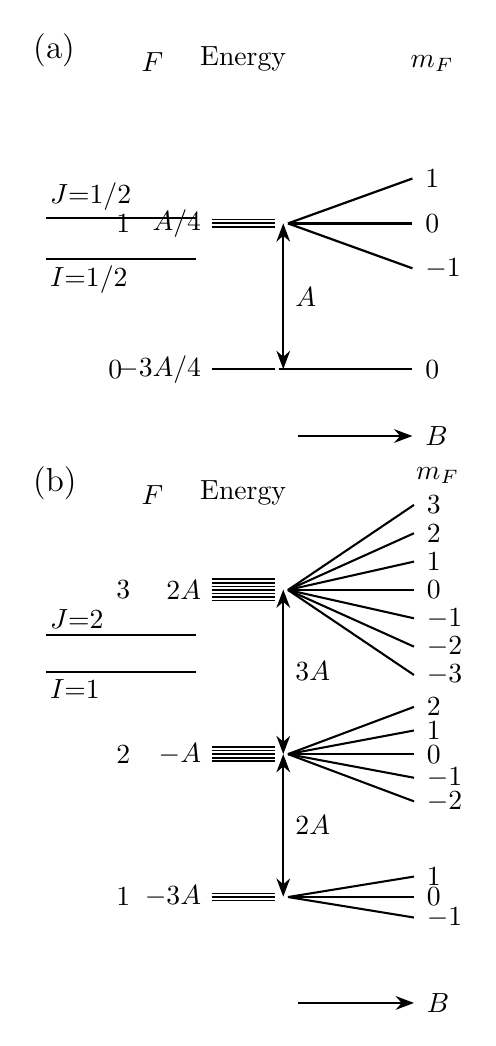
\begin{tikzpicture}[line width=0.8pt,>=Stealth]
% ---------- (a) I=1/2, J=1/2 ----------
\node[anchor=north west,inner sep=2pt] at (-0.6,5.05) {\large (a)};
\node[anchor=south] at (1.0,4.35) {$F$};
\node[anchor=south] at (2.15,4.35) {Energy};
\node[anchor=south] at (4.55,4.35) {$m_F$};
% 左侧 J、I 参考线
\draw[line width=0.7pt] (-0.35,2.62) -- (1.55,2.62);
\node[anchor=south west,inner sep=1pt] at (-0.35,2.66) {$J{=}1/2$};
\draw[line width=0.7pt] (-0.35,2.10) -- (1.55,2.10);
\node[anchor=north west,inner sep=1pt] at (-0.35,2.06) {$I{=}1/2$};
% F=1（3 重线，能量 A/4）
\foreach \y in {2.500,2.550,2.600} \draw[line width=0.7pt] (1.75,\y) -- (2.55,\y);
\node[anchor=east,inner sep=2pt] at (0.80,2.55) {$1$};
\node[anchor=east,inner sep=2pt] at (1.70,2.55) {$A/4$};
% F=0（单线，能量 -3A/4）
\draw[line width=0.7pt] (1.75,0.70) -- (2.55,0.70);
\node[anchor=east,inner sep=2pt] at (0.70,0.70) {$0$};
\node[anchor=east,inner sep=2pt] at (1.70,0.70) {$-3A/4$};
% A 间隔
\draw[<->,line width=0.8pt] (2.66,2.55) -- (2.66,0.70);
\node[anchor=west,inner sep=2pt] at (2.73,1.62) {$A$};
% 磁场中 m_F 分裂
\foreach \mf/\ye in {1/3.12,0/2.55,-1/1.98}
  \draw[line width=0.8pt] (2.72,2.55) -- (4.30,\ye);
\draw[line width=0.8pt] (2.60,0.70) -- (4.30,0.70);
\foreach \mf/\ye in {1/3.12,0/2.55,-1/1.98}
  \node[anchor=west,inner sep=2pt] at (4.38,\ye) {$\mf$};
\node[anchor=west,inner sep=2pt] at (4.38,0.70) {$0$};
% B 轴
\draw[->,line width=0.8pt] (2.85,-0.15) -- (4.30,-0.15);
\node[anchor=west,inner sep=2pt] at (4.38,-0.15) {$B$};
% ---------- (b) I=1, J=2 ----------
\begin{scope}[shift={(0,-7.0)}]
\node[anchor=north west,inner sep=2pt] at (-0.6,6.55) {\large (b)};
\node[anchor=south] at (1.0,5.85) {$F$};
\node[anchor=south] at (2.15,5.85) {Energy};
\node[anchor=south] at (4.62,6.12) {$m_F$};
% 左侧 J、I 参考线
\draw[line width=0.7pt] (-0.35,4.32) -- (1.55,4.32);
\node[anchor=south west,inner sep=1pt] at (-0.35,4.36) {$J{=}2$};
\draw[line width=0.7pt] (-0.35,3.85) -- (1.55,3.85);
\node[anchor=north west,inner sep=1pt] at (-0.35,3.81) {$I{=}1$};
% F=3（7 重线，能量 2A）
\foreach \y in {4.760,4.805,4.850,4.895,4.940,4.985,5.030} \draw[line width=0.6pt] (1.75,\y) -- (2.55,\y);
\node[anchor=east,inner sep=2pt] at (0.80,4.90) {$3$};
\node[anchor=east,inner sep=2pt] at (1.70,4.90) {$2A$};
% F=2（5 重线，能量 -A）
\foreach \y in {2.720,2.765,2.810,2.855,2.900} \draw[line width=0.6pt] (1.75,\y) -- (2.55,\y);
\node[anchor=east,inner sep=2pt] at (0.80,2.81) {$2$};
\node[anchor=east,inner sep=2pt] at (1.70,2.81) {$-A$};
% F=1（3 重线，能量 -3A）
\foreach \y in {0.950,0.995,1.040} \draw[line width=0.6pt] (1.75,\y) -- (2.55,\y);
\node[anchor=east,inner sep=2pt] at (0.80,1.00) {$1$};
\node[anchor=east,inner sep=2pt] at (1.70,1.00) {$-3A$};
% 间隔箭头 3A 与 2A
\draw[<->,line width=0.8pt] (2.66,4.90) -- (2.66,2.81);
\node[anchor=west,inner sep=2pt] at (2.73,3.86) {$3A$};
\draw[<->,line width=0.8pt] (2.66,2.81) -- (2.66,1.00);
\node[anchor=west,inner sep=2pt] at (2.73,1.91) {$2A$};
% 磁场中分裂：F=3 -> 7 支
\foreach \mf in {3,2,1,0,-1,-2,-3}
  \draw[line width=0.75pt] (2.72,4.895) -- (4.32,{4.895+0.36*\mf});
% F=2 -> 5 支
\foreach \mf in {2,1,0,-1,-2}
  \draw[line width=0.75pt] (2.72,2.810) -- (4.32,{2.810+0.30*\mf});
% F=1 -> 3 支
\foreach \mf in {1,0,-1}
  \draw[line width=0.75pt] (2.72,0.995) -- (4.32,{0.995+0.26*\mf});
% m_F 标签
\foreach \mf in {3,2,1,0,-1,-2,-3}
  \node[anchor=west,inner sep=2pt] at (4.40,{4.895+0.36*\mf}) {$\mf$};
\foreach \mf in {2,1,0,-1,-2}
  \node[anchor=west,inner sep=2pt] at (4.40,{2.810+0.30*\mf}) {$\mf$};
\foreach \mf in {1,0,-1}
  \node[anchor=west,inner sep=2pt] at (4.40,{0.995+0.26*\mf}) {$\mf$};
% B 轴
\draw[->,line width=0.8pt] (2.85,-0.35) -- (4.32,-0.35);
\node[anchor=west,inner sep=2pt] at (4.40,-0.35) {$B$};
\end{scope}
\end{tikzpicture}
\end{document}
